\documentclass{article}
\usepackage{hyperref}
\usepackage{amsmath}
\usepackage{graphicx}
\usepackage{caption}
\usepackage{subcaption}
\usepackage[section]{placeins}
\renewcommand{\thesubsection}{\thesection.\alph{subsection}}
\usepackage{listings}
\usepackage{amssymb}

\title{\bf{CSE397: Assignment \#2}}
\author{Nicholas Malaya \\ Department of Mechanical Engineering \\
Institute for Computational Engineering and Sciences \\ University of
Texas at Austin} \date{} 

\begin{document}
\maketitle

\newpage
\section{Problem 1}

\subsection{Find and classify all stationary points}


\begin{figure}[!htb]
  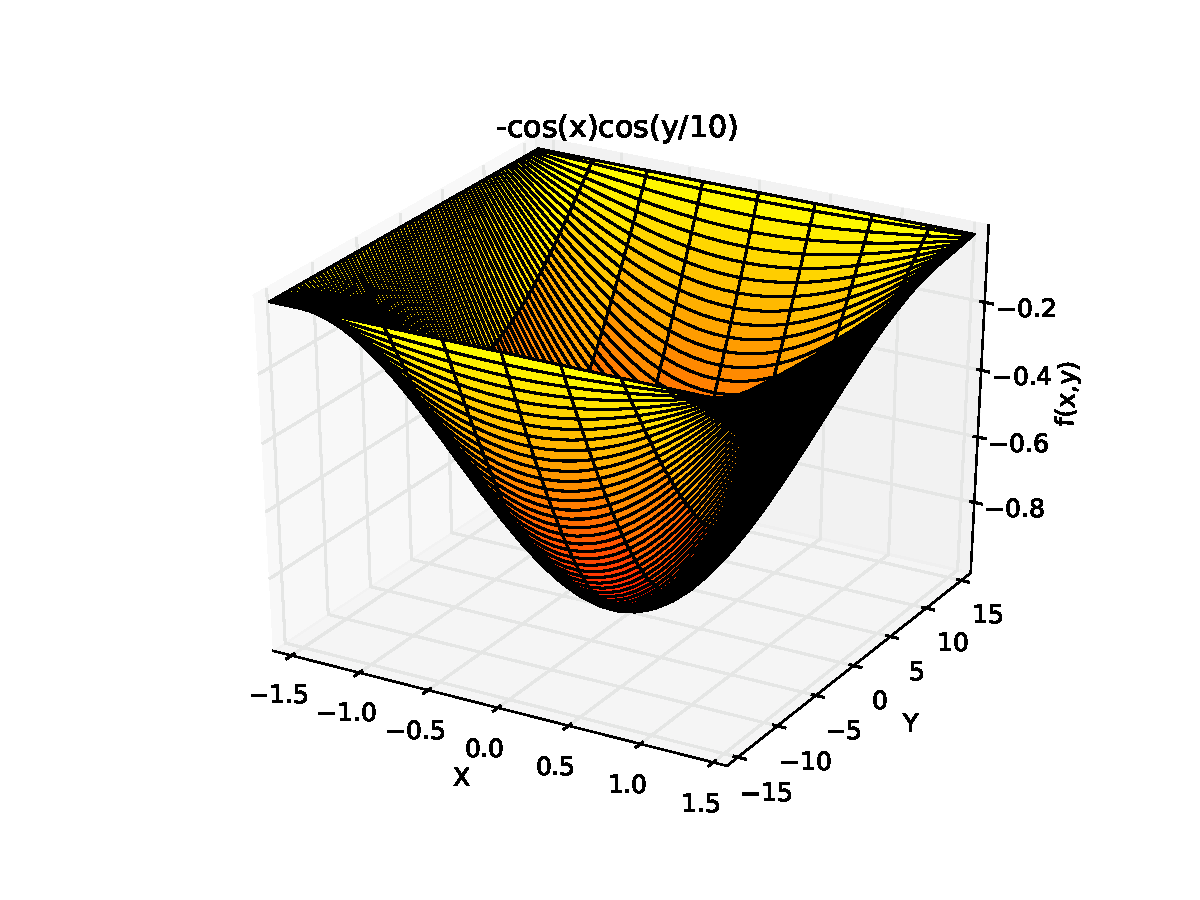
\includegraphics[scale=.5]{figs/1_3d.pdf}
  \label{fig:3d}
  \caption{The topology of -cos(x)cos(y/10) in the domain.} 
\end{figure}

Figure one shows a clear stationary point at (0,0). In addition, we are
seeking all points where $\nabla f = 0$.  The gradient of $\nabla f =
(\text{sin}(x)\text{cos}(y/10),\frac{\text{cos}(x)}{10}\text{sin}(y/10))$. Solving
$\text{sin}(x)\text{cos}(y/10) = 0$  and
$\frac{\text{cos}(x)}{10}\text{sin}(y/10) = 0$ shows that while the
directional derivative of x is zero at $y \pm \frac{10 \pi}{2}$ and the
y-derivative is zero at $x \pm \frac{\pi}{2}$, the entire gradient is
only zero at (0,0). Thus, this is the only fixed point in the region we
are considering. 

\subsection{Find the region where the Hessian Matrix of f(x,y) is positive definite.}

\subsection{Derive expressions for the search directions}

\subsection{Write a program that performs both steepest descent and a
  Newton Iteration}


% \subsection{$T_{\text{SVD}}$}


% \begin{figure}[!htb]
%         \centering
%         \begin{subfigure}[bh]{0.45\textwidth}
%                 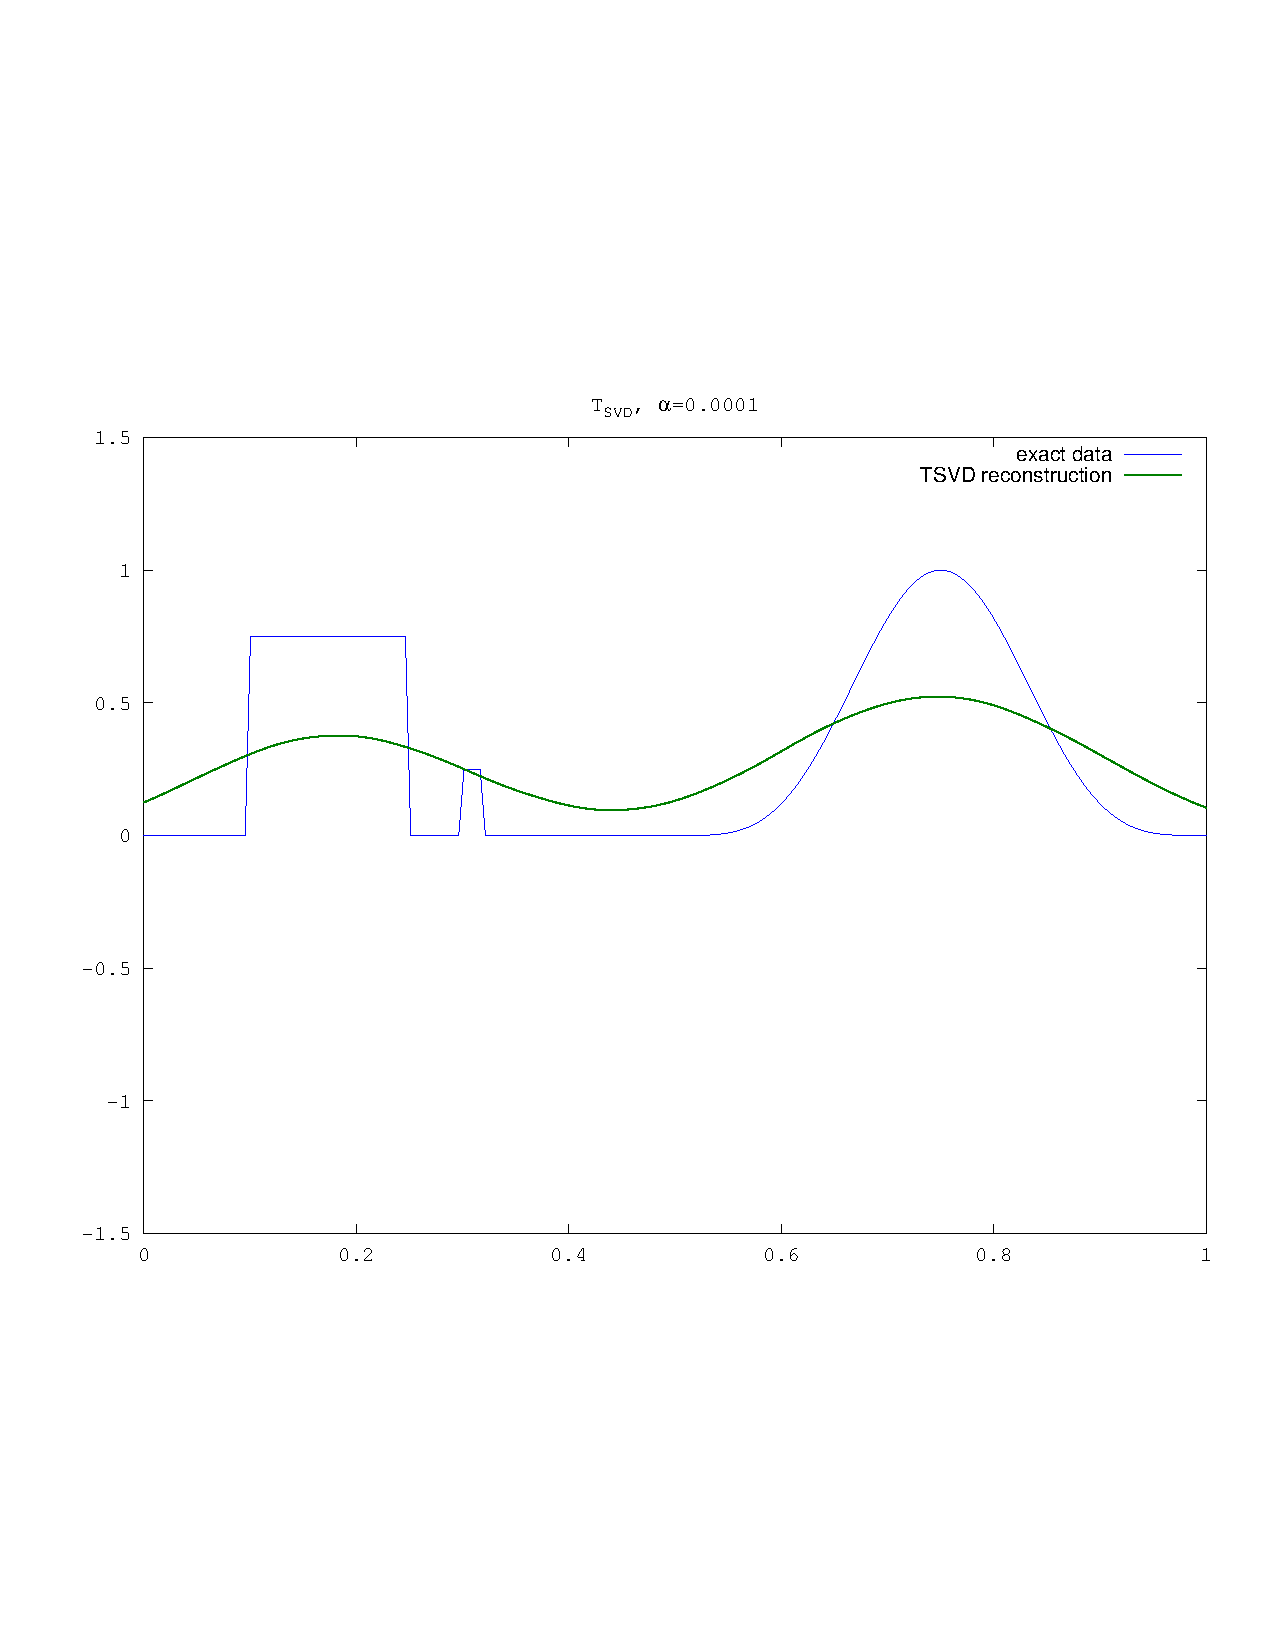
\includegraphics[width=\textwidth]{plots/tsvd0001.pdf}
%                 \caption{$\alpha=0.0001$}
%         \end{subfigure}%
%         \begin{subfigure}[bh]{0.45\textwidth}
%                 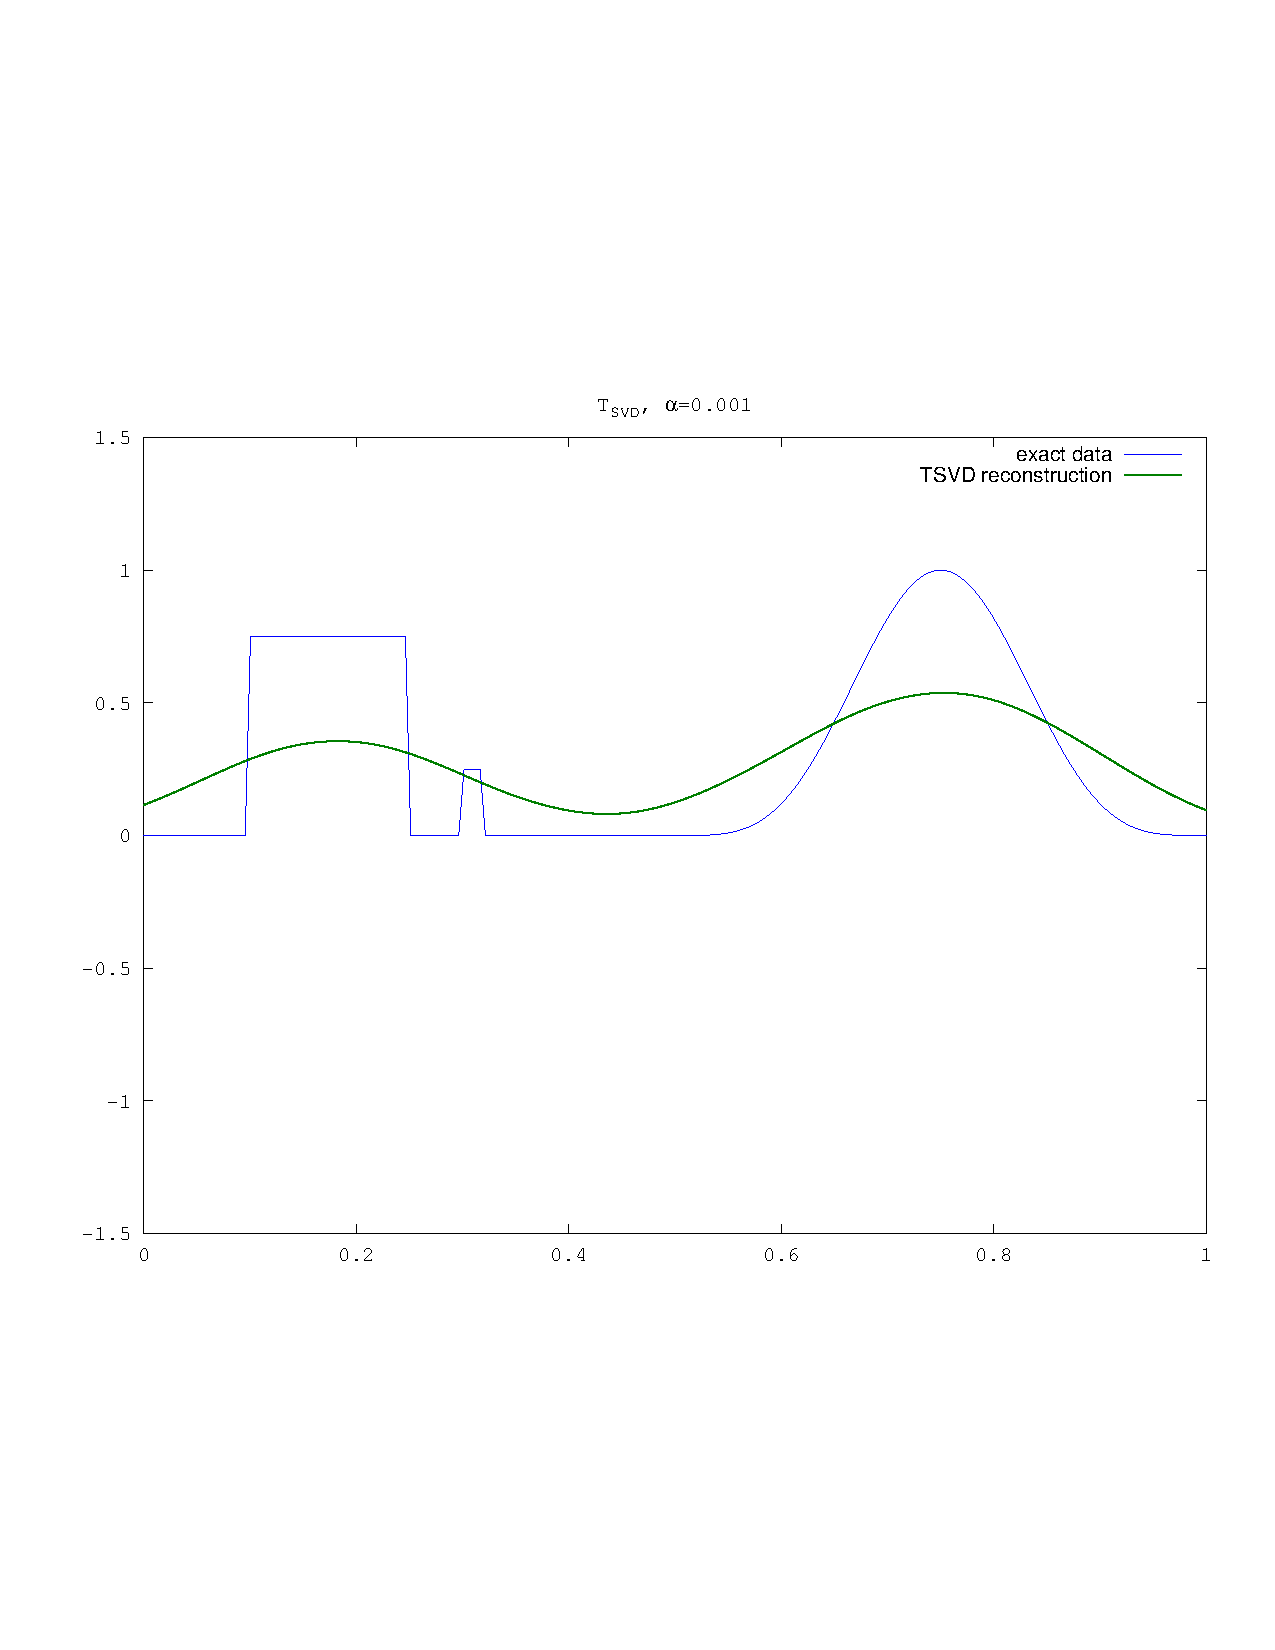
\includegraphics[width=\textwidth]{plots/tsvd001.pdf}
%                 \caption{$\alpha=0.001$}
%         \end{subfigure}
%         \centering
%         \begin{subfigure}[bh]{0.45\textwidth}
%                 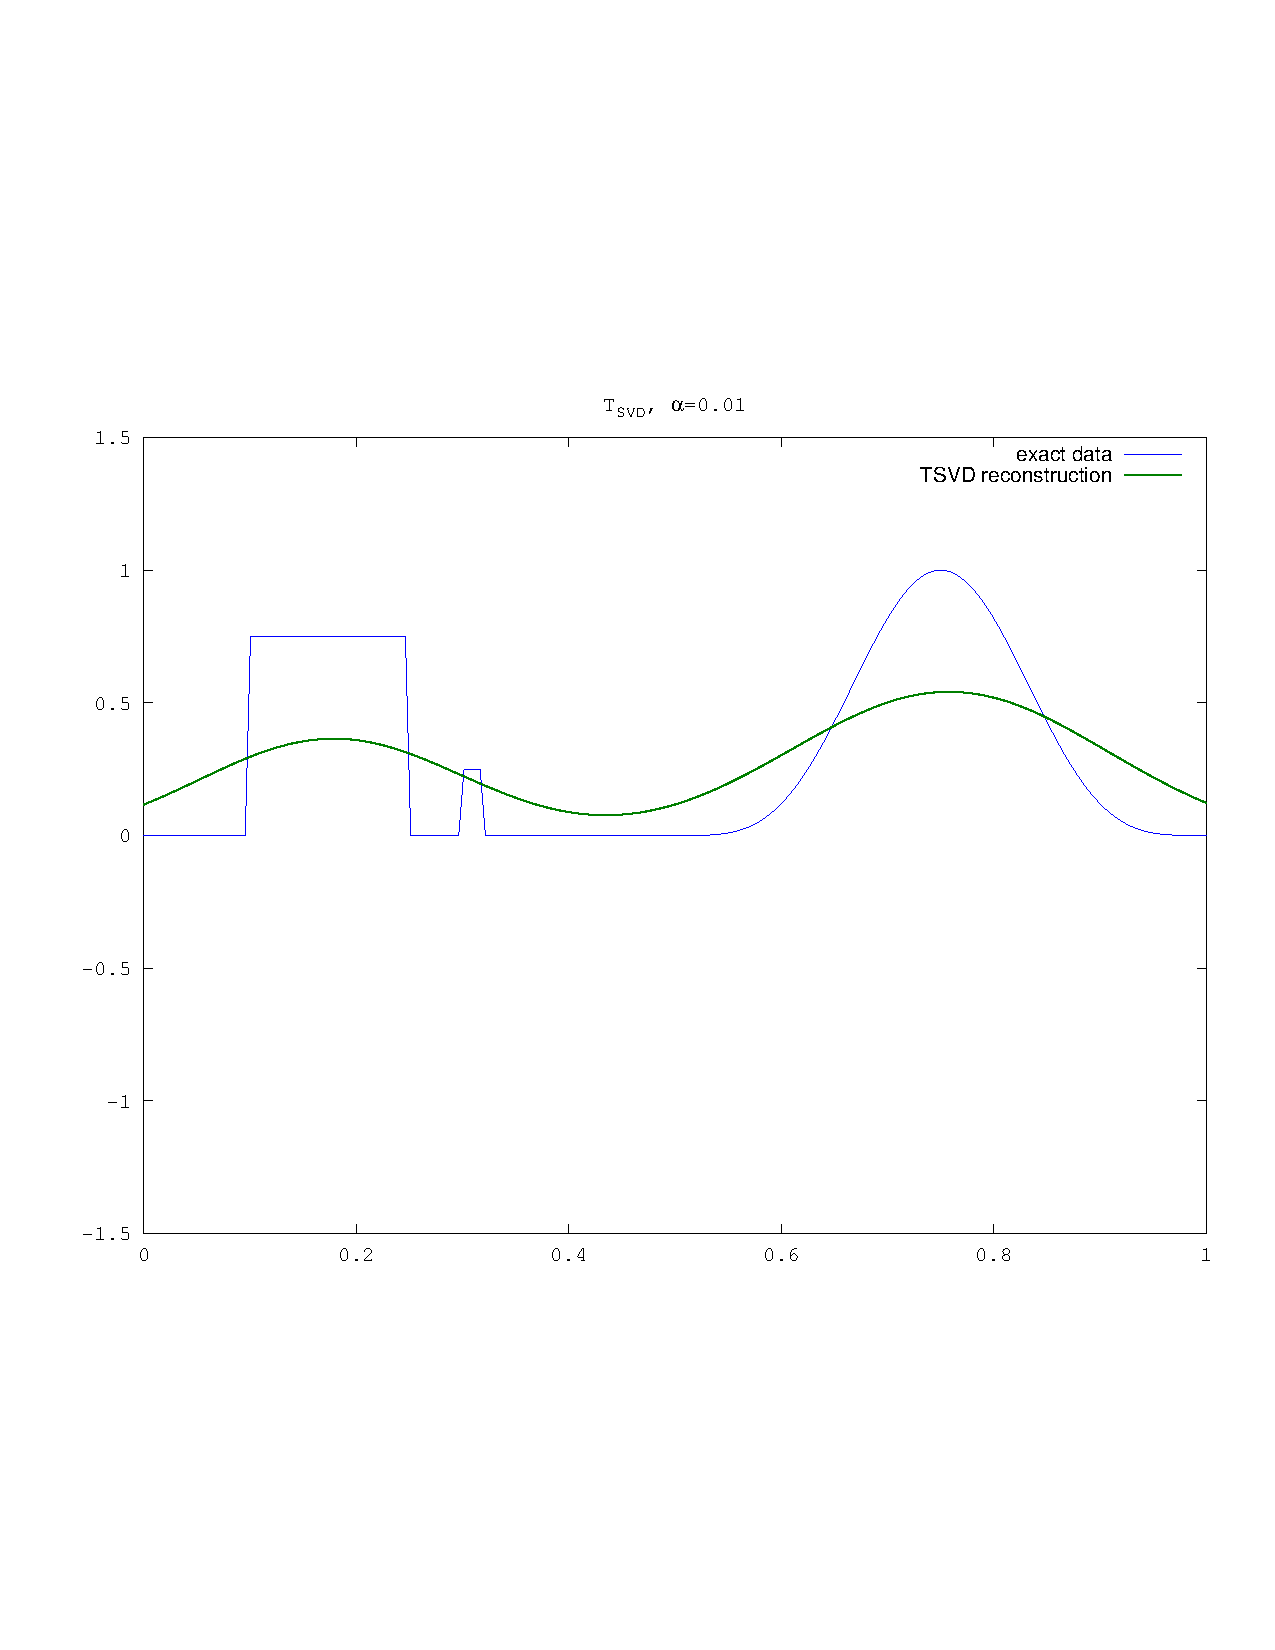
\includegraphics[width=\textwidth]{plots/tsvd01.pdf}
%                 \caption{$\alpha=0.1$}
%         \end{subfigure}%
%         \begin{subfigure}[bh]{0.45\textwidth}
%                 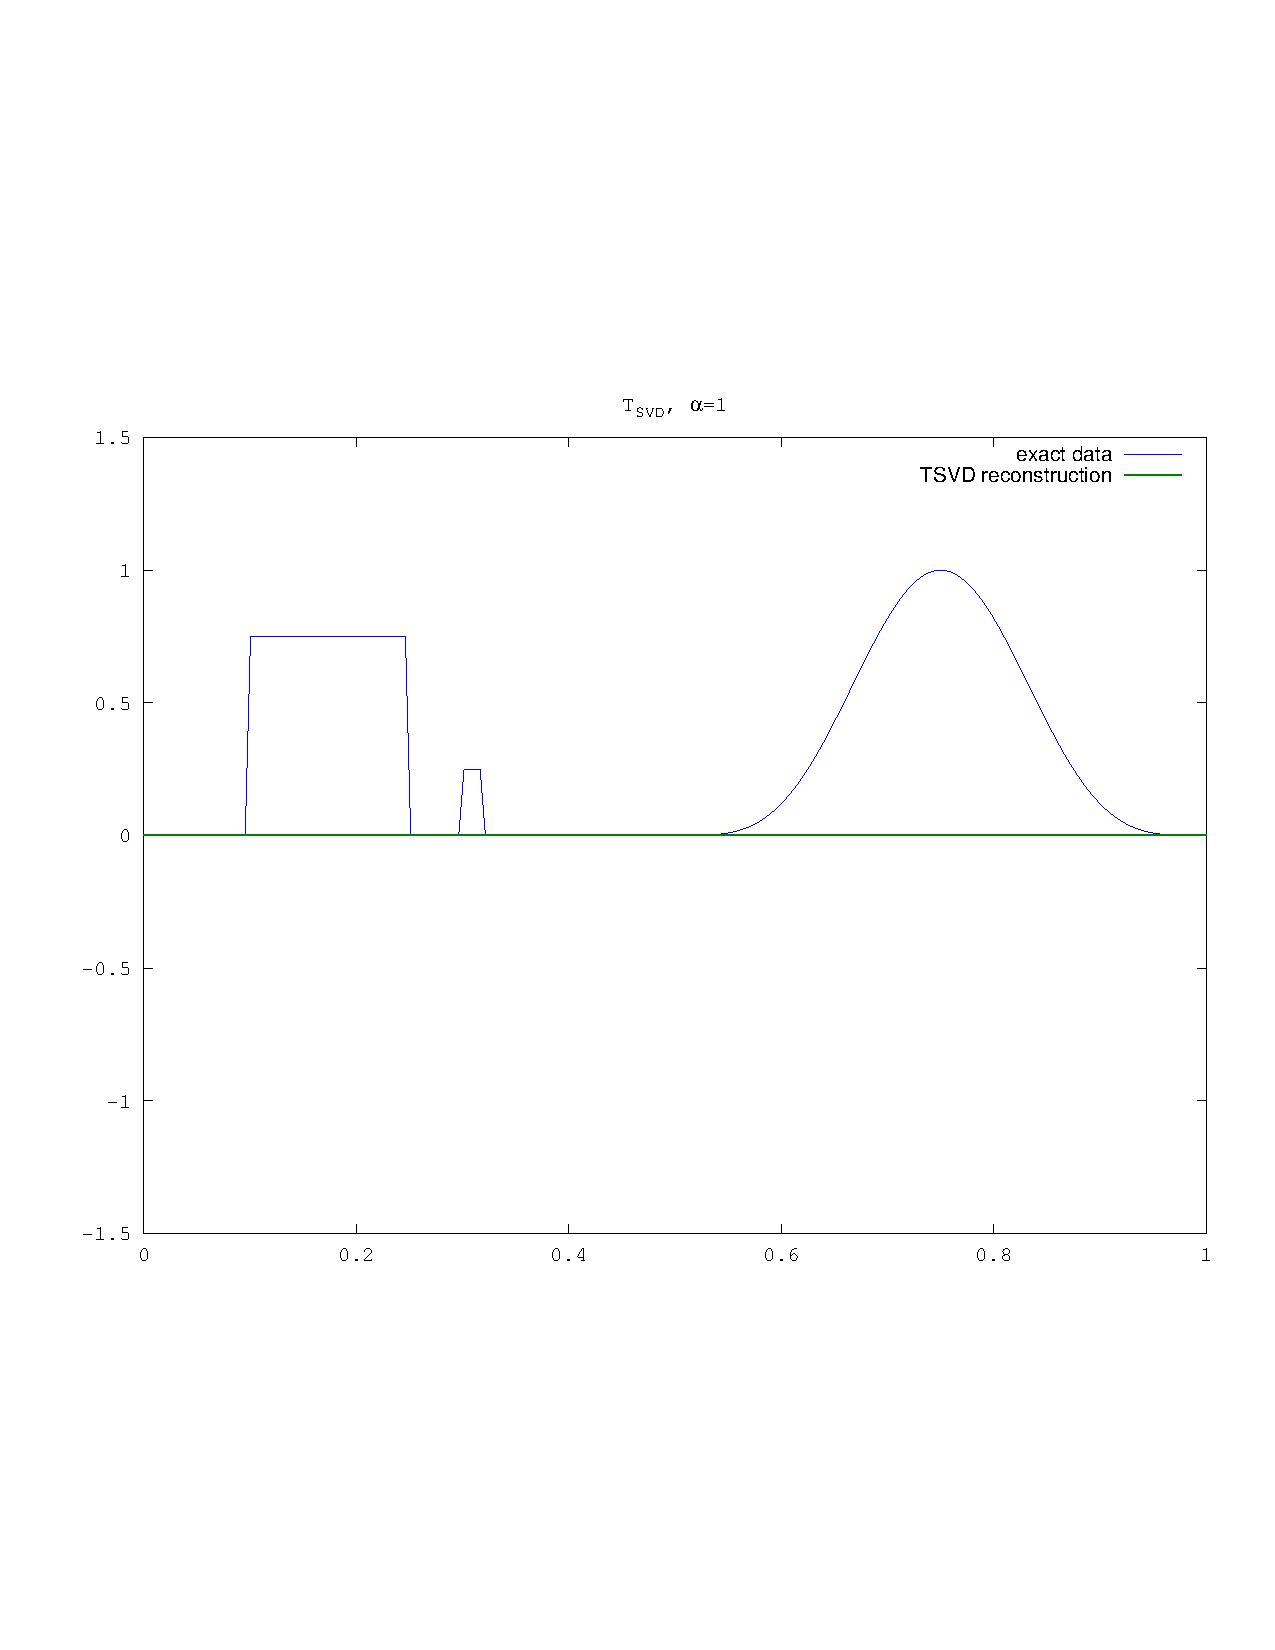
\includegraphics[width=\textwidth]{plots/tsvd1.pdf}
%                 \caption{$\alpha=1.0$}
%         \end{subfigure}
%         \caption{$T_{\text{SVD}}$ at varying values of $\alpha$.}
%         \label{fig:svd}
% \end{figure}

% Figure \ref{fig:svd} plots the solution to the inverse problem using
% Truncated SVD at several different values of $\alpha$, the
% regularization parameter. We can see that actually, the filter nicely
% regularizing the inverse problem even for small values of $\alpha$. It
% is only for the largest value of $\alpha$ that the parameter is obviously
% too large, at which point almost all the frequencies are filtered out,
% and the solution to the inverse problem is constant and zero. 

% As expected, none of the solutions capture any of the very fine (high
% frequency) features of the original data. 

% \subsection{L-Curve}

% % \begin{figure}[!htb]
% %   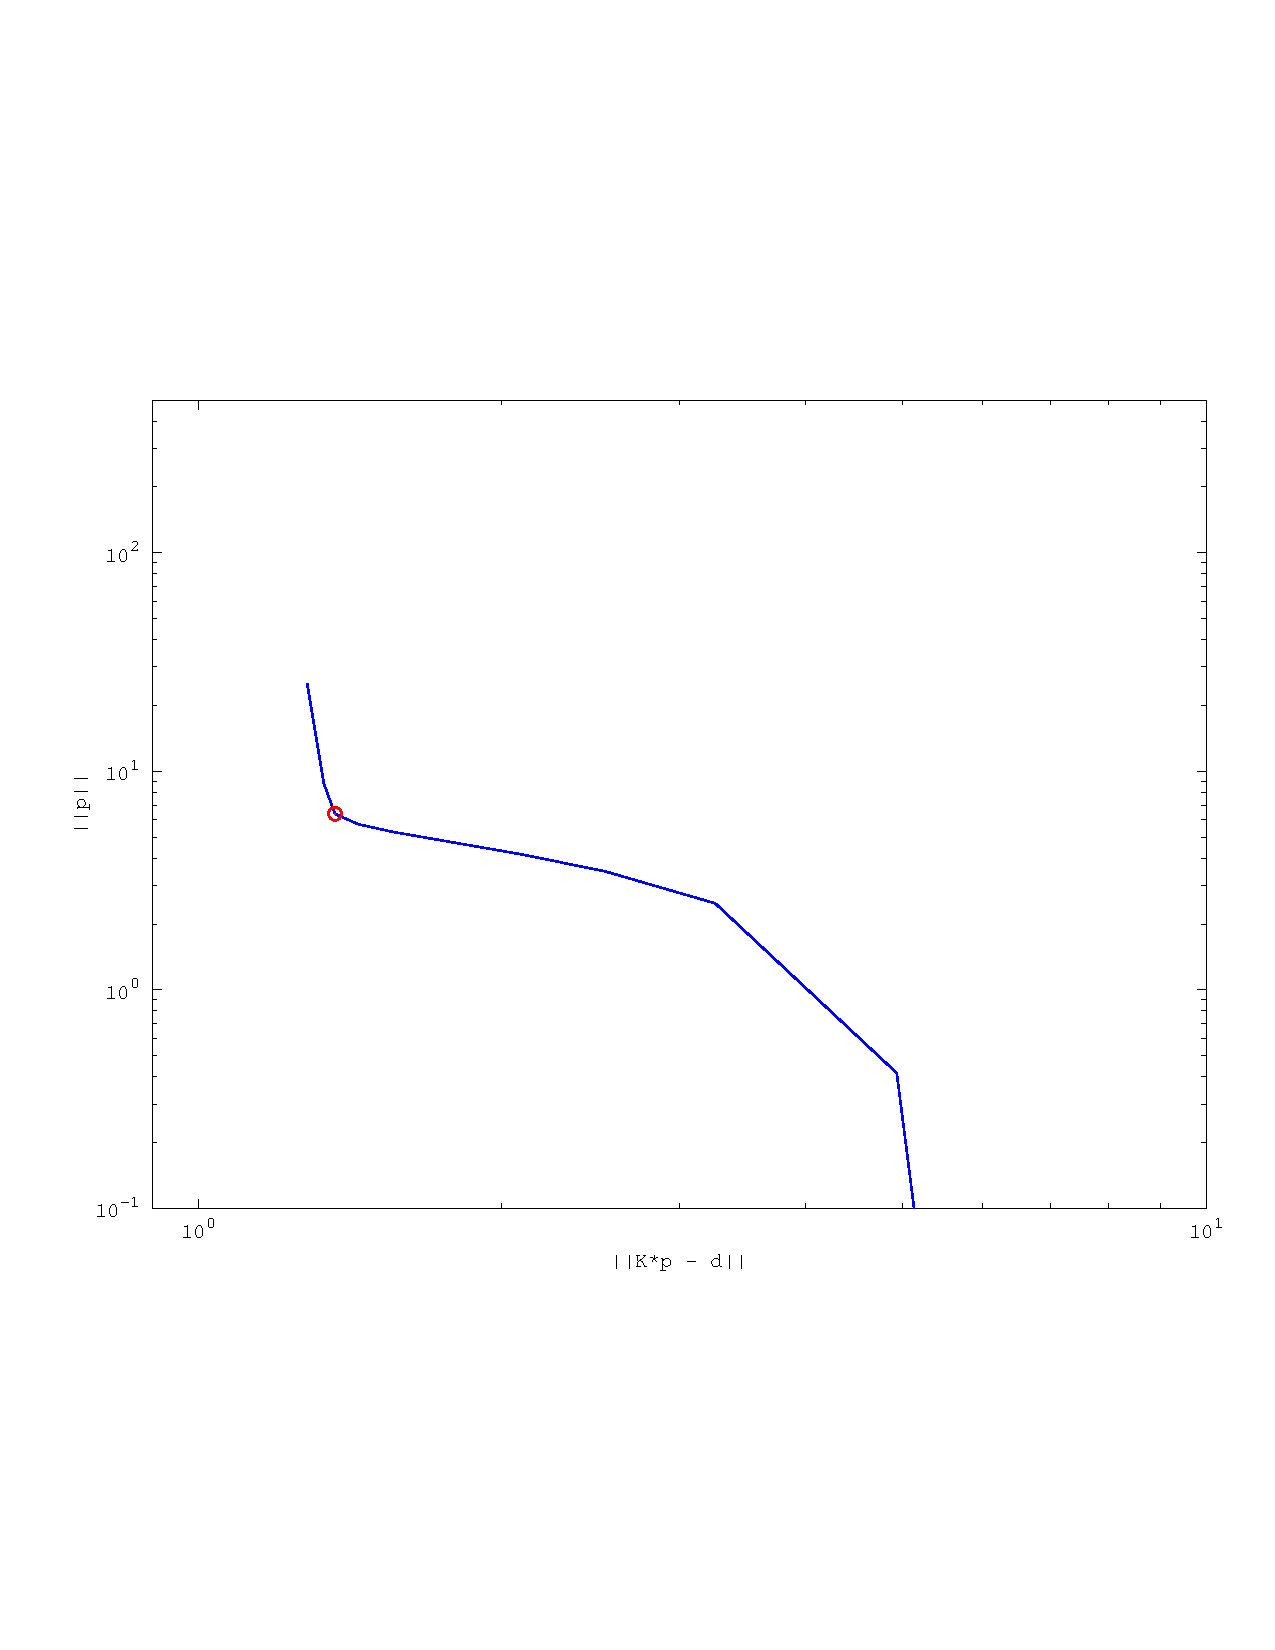
\includegraphics[scale=.6]{plots/L-curve.pdf}
% %   \caption{The L-curve} 
% %  \label{fig:lcurve}
% % \end{figure}

% Figure \ref{fig:lcurve} plots the results of the L-curve criterion. The
% red dot plotted is at 0.01. This is approximately the ``optimal'' value
% of regularization, which is generally consistent with the observations
% of the previous plots. 

\section{Problem 2}

\subsection{Show that the two problems have the same minimizers}

We can see that the problems must have the same minimizers
(e.g. $x^\star$) because $\beta$ is just a scale factor, and our solution
should be invariant to homogeneous linear mappings. 

Intuitively, if we multiply our function at each point by 10x, then 
the lowest point should remain in the same place (and likewise, for the
max). 

More formally speaking, our first order necessary conditions for a local
minimizer, $x^\star$, require that if $x^\star$ is a local minimizer of
$f_2(x)$, then $g_2(x^\star) = 0 $ at the local minimizer. 

However, $f_2(x) = \beta f_1(x)$. Therefore,  $f_2(x^\star) = \beta
f_1(x^\star)$, and $g_1(x^\star) = g_2(x^\star) = 0 $. Therefore, the
gradient is also zero at $x^\star$ for $f_1$.

\subsection{Compare Steepest Descent and Newton Directions at $x_0 \in \mathbb{R}$}

\begin{align*}
 p_k&=-g_k = -\nabla f_k\\
 p_{k,1}&=-g_{k,1}\\
 p_{k,2}&=-g_{k,2} = -\beta g_{k,1}
\end{align*}

Thus, 
\begin{equation}
p_{k,2} \ne p_{k,1}
\end{equation}
for steepest descent: the search directions
vary by a scale factor. However, using Newton's method, the first search
direction is,
\begin{align*}
 H_k p_k&=-g_k \\
 H_{k,1} p_{k,1}&=-g_{k,1}\\
\end{align*}
And the second is,
\begin{align*}
 H_{k,2} p_{k,2}&=-g_{k,2}\\
 \beta H_{k,1} p_{k,2}&=- \beta g_{k,1}\\
 H_{k,1} p_{k,2}&=-g_{k,1}
\end{align*}
And therefore, 
\begin{equation}
p_{k,2} = p_{k,1}
\end{equation}
Thus, Newton's method is insensitive to the scale of the underlying
problem. Steepest decent on the other hand, does depent on the scale of
the underlying problem, and therefore it is not possible to make a good
initial step length, $\alpha$.

\subsection{Multidimensional expansion}

The result from the previous section is generalizable to
multi-dimensions. Now, instead of $\beta$ we have B, a matrix of
positive elements that scale the function f(x) that we are trying to
minimize. 

\begin{equation}
 Bg(x) = 0
\end{equation}
As before, our Newton step is insensitive to the scale of the system we
are solving, 
\begin{align*}
 H_{k} p_{k}&=-g_{k}\\
 B H_{k} p_{k}&=- B g_{k}\\
 (B^{-1}B)H_{k} p_{k}&=-(B^{-1}B)g_{k}
 H_{k} p_{k}&=-g_{k}\\
\end{align*}
This is because the same scale factor will ``push-through'' the Hessian
Matrix, e.g. 
\begin{equation}
H(x) = \nabla\nabla B f(x) = B \nabla\nabla f(x) 
\end{equation}
Thus, Newton's method is affine invariant, e.g. independent of linear
changes of coordinates. 

\section{Problem 3}

Write a program to minimize a quartic form -- a homogeneous polynomial
of degree four. 

\subsection{Code}

\subsection{Compare the performance between Newton and Steepest Descent}

\subsection{Experiment with different choices of $\eta$}

Verify the theoretical convergence rates for these different choices. 

\end{document}